\section{Single-Phase RANS Computation}
%
\subsection{What you Will Learn}
%
In this part of the tutorial you will learn how to set-up, run, and post-process the results of a steady-state single phase RANS calculation for the Arnason pipe generated in the previous Section, using the CFDStudy module in \salome. You will also learn how to integrate user defined functions into a \CS calculation. The user defined functions will be used to specify the inlet boundary conditions. Probes will also be set in the computational domain and used in the analysis to verify that steady-state, converged results are obtained.
%
\subsection{Setting up the CFD Simulation}
%
The CFD case is set-up and run from the CFDStudy module (Section \ref{lag:create_CS_struct}). 

In the CFDStudy module, launch the CFDStudy GUI and verify that the case directory structure has been correctly recognised by clicking on the \textbf{Identity and Paths} folder in the tree menu.  If the case directory is correct you can continue.  If not, you will need to set the correct directory.  Then, save the CFD data file. By default, its name will be setup.xml.

You can now proceed with setting up the case, following the top-down order of the folders in the left-hand column, starting with the mesh.

\subsubsection{Selecting the Volume Mesh}

Go to the {\color{eblue} \bf Mesh} section  and, in the \menu{List of meshes} add the mesh ‘Mesh\_ARNASON.med’. This is done by clicking on the \keys{$+$} icon in the panel and selecting the appropriate mesh in the MESH directory, as shown in \figurename~\ref{lag:import_mesh}.  No further input is necessary for the volume mesh.
%
\begin{figure}[H]
\centering
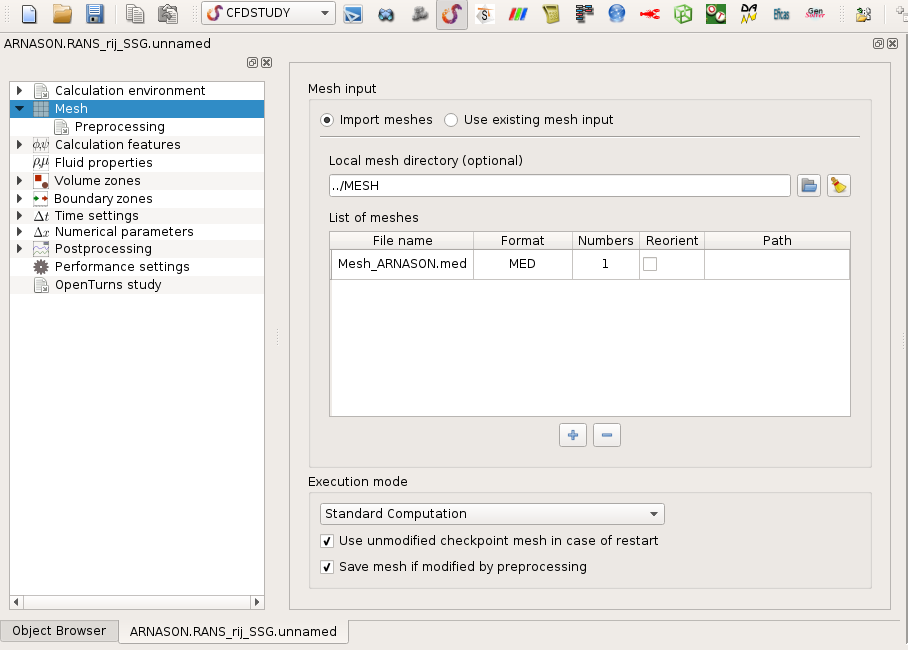
\includegraphics[width=0.6\textwidth]{\IMAGES/Part4_RANS/import_mesh.png}
\caption{Importing the mesh.}\label{lag:import_mesh}
\end{figure}
%

\subsubsection{Calculation features}

In the \textbf{Calculation features} section, leave all options to their default values, i.e. only \textbf{Standard Eulerian single phase} is selected.

In the \textbf{Turbulence models} sub-section, change the \textit{Turbulence model} to \textit{Rij-epsilon SSG}.  In the \textbf{Advanced Options} menu, ensure that the wall function type is set to ‘Two scales model’ and that ‘Gravity terms in the turbulence equations’ is selected.

In the \textbf{Body forces} sub-section, set the acceleration of gravity by entering the value ‘$-9.81 m/s^2$’ for its component in the vertical (Z) direction in the ‘Gravity’ panel.

Now you can go to the \textbf{Fluid Properties} section.

\subsubsection{Physical Properties}

Given that the flow field is incompressible, the physical properties of the fluid are constant for a constant fluid temperature of \textbf{$10^{\circ}C$}.  Specify the value of each fluid property as shown in \figurename~\ref{lag:fluid_prop_gui}.
%
\begin{figure}[H]
\centering
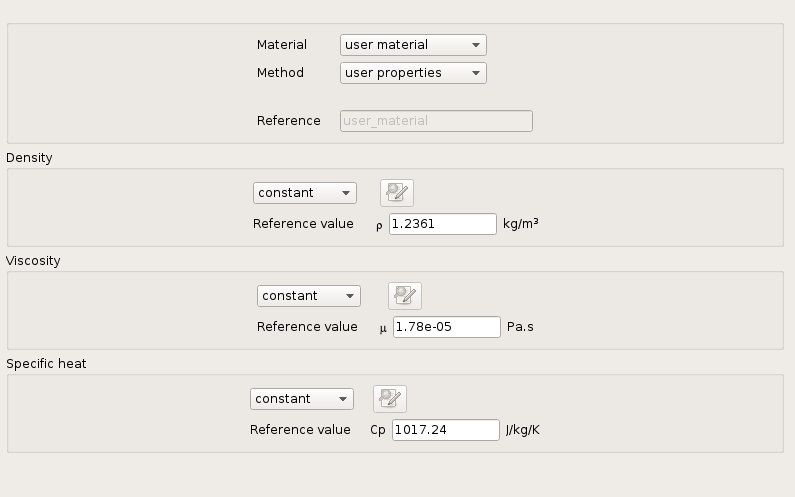
\includegraphics[width=0.6\textwidth]{\IMAGES/Part4_RANS/Fluid_properties.png}
\caption{Specifying the fluid properties.}\label{lag:fluid_prop_gui}
\end{figure}
%


No other settings are required in this folder.  You can now move to the \textbf{Initialization} under the \textbf{Volume zones} section.

\subsubsection{Initialization}

The initial values for the velocity are defined in the ‘Initialization’ tab. The flow is initially stagnant by default.

No other settings are required in this folder.  You can now move to the ‘Boundary zones’ section.

\subsubsection{Boundary zones}\label{lag:inlet_outlet_BCs}

Three boundary conditions are used in this study: inlet, wall and outlet.  These conditions are listed in \tablename~\ref{lag:bc_air_part}.   The inlet boundary condition will be defined in the ‘cs\_user\_boundary\_condition’ subroutine so it does not need to be generated here (see \ref{lag:code_inlet}).

First, create the 'wall' and 'outlet' boundary regions by selecting the wall and outlet group in \salome object browser and by clicking on \keys{Add from Salome} (\figurename~\ref{lag:def_bc}).  Finally, change the type ('Nature') of the boundary to ‘outlet’ for the outlet boundary but leave the type of the wall boundary condition as ‘wall’.
%
\begin{figure}[H]
\centering
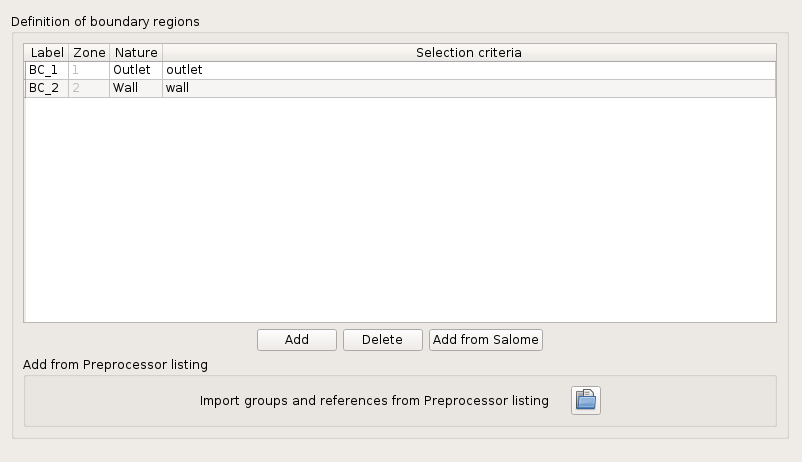
\includegraphics[width=0.6\textwidth]{\IMAGES/Part4_RANS/def_bc.png}
\caption{Defining the boundary conditions.}\label{lag:def_bc}
\end{figure}
%
Having defined their type, the values to apply at each boundary could now be specified.  However, as the default values are used in this tutorial, no further specification is necessary.  To check the default values, select the ‘Boundary conditions’ sub-folder and click on the boundary of interest.

No other settings are required in this folder. You can now go to the ‘Numerical parameters’ folder.

\subsubsection{Numerical Parameters}

In the \keys{Equation parameters} sub-folder, the \keys{Solver} panel shows that pressure, velocity, turbulent kinetic energy and turbulent kinetic energy dissipation are solved for. In order to decrease overall computation time, it is possible to decrease the solver precision by setting the convergence criterium to $10^{-5}$ for each variable, except for pressure, without having an impact on solution quality.

In the \keys{Time step} panel, set the time step to 0.01s and the number of iterations to 850.  For this tutorial, this number of iterations is sufficient to reach a steady-state flow solution.

\subsubsection{Calculation Control}

In the \keys{Calculation control} folder, select the \keys{Output control} sub-folder and go into the \keys{Monitoring Points} panel.  Click on the \keys{$+$} icon to add a probe, then enter the coordinate of the probe.  Repeat this procedure for the probes of your choice.  Monitoring probes can be useful to check the convergence of the simulation and it is recommended that monitoring points are specified along the axis of the pipe after the particle injection point.  The monitoring points used for this tutorial are shown in \figurename~\ref{lag:monitoring}. Select the \keys{csv} format in order to be able to open the output files in \paravis.
%
\begin{figure}[H]
\centering
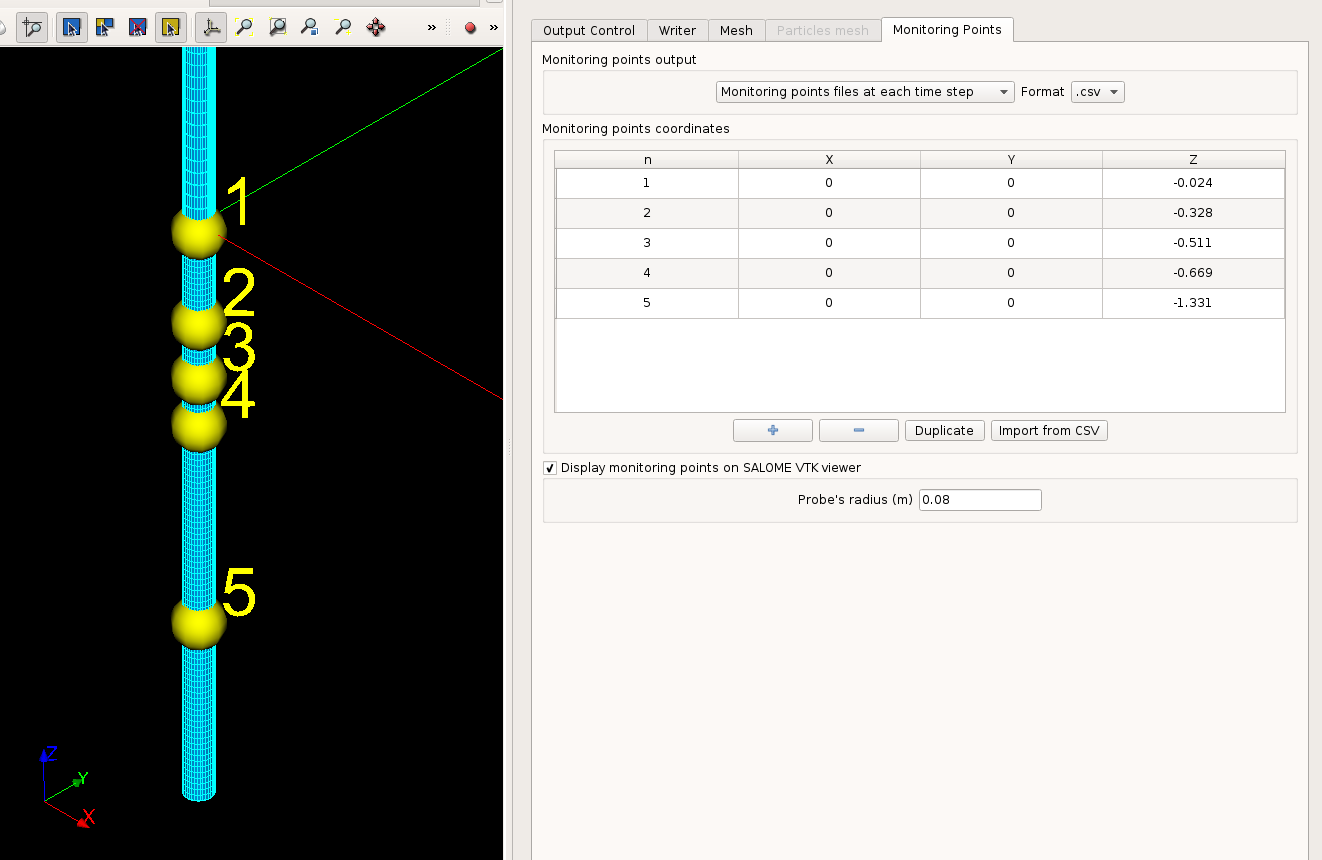
\includegraphics[width=\textwidth]{\IMAGES/Part4_RANS/monitoring_points_v2.png}
\caption{Monitoring points.}\label{lag:monitoring}
\end{figure}
%
The \CS calculation is now fully specified from the standpoint of the GUI and the \CS case 'xml' file should be saved.  However, prior to running the simulation, the inlet boundary condition still needs to be specified.  A parabolic law defining the $V_z$ velocity component needs to be coded in the ‘cs\_user\_boundary\_conditions.f90’ subroutine.  This step is described next.

\subsubsection{Programming the Inlet Boundary Condition}\label{lag:code_inlet}

To begin with, copy the sample file ‘cs\_user\_boundary\_conditions-base.f90’ from the tutorial $/../ARNASON/\\RANS\_rij\_SSG/SRC/EXAMPLES$ directory to your SRC directory.  This is done in order to create a local copy which you will be able to customise and which will be automatically recompiled and linked to the ‘cs\_solver’ executable at run time.

Once copied, open your local version of the file by a right-click on it in the object browser or by using the text editor of your choice.  This subroutine contains several examples of different boundary conditions that can be used by \CS.  In this tutorial, you will customise ‘Example 1’ with your own implementation of the $V_z$ velocity as a function of radius (Eq. \ref{lag:bc_air_part}).  To keep your code clean, you may remove all the other examples from the file.  The customised code is available with this tutorial and is already commented.  Here we describe the main parts of this user coding and the logic behind them.
%
\begin{enumerate}
\item Declare your own local variables at the top of the subroutine, either as double precision real values or integer values
\item Initialise your own local variables
\item Use the subroutine ‘getfbr’ to select the faces attached to the ‘inlet’ boundary condition
\item Cycling through the boundary faces.
\begin{enumerate}
\item Apply the type ‘entre’ to all boundary faces
\item Calculate the $V_z$ velocity component and the turbulence based on the hydraulic diameter
\end{enumerate}
\end{enumerate}
%
\subsection{Running and Analysing the Simulation}

\subsubsection{Running the Simulation}

To launch the simulation, click on the {\color{eblue} \bf Run or submit solver} button as shown below:

\begin{figure}[H] 
\centering
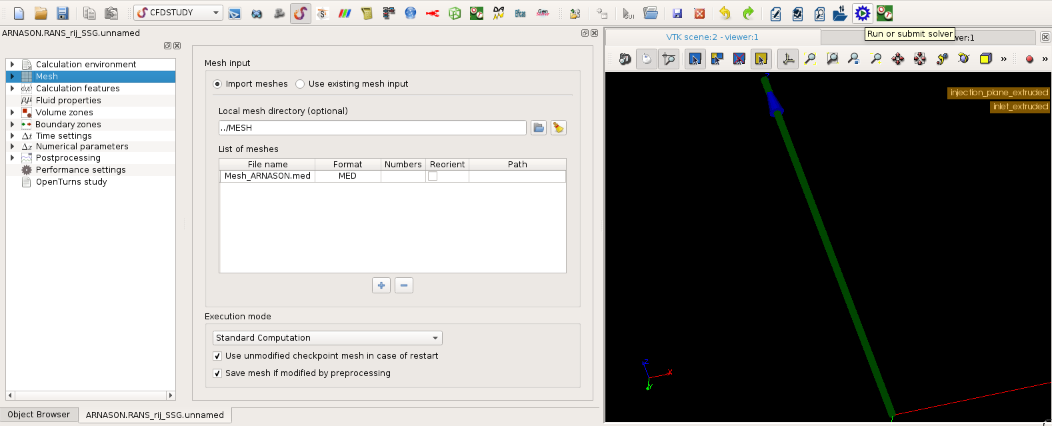
\includegraphics[width=\textwidth]{\IMAGES/Part4_RANS/run_submit_solver.png} 
\caption{Run}
\label{lag:cap1_run}
\end{figure}

A window will open where you can specify the run options.

All options except the number of processes are let to their default values:
%
\begin{itemize}
\item ‘runcase’ for the ‘Script file’
\item ‘1’ for the number of threads per process
\item build type to '[default]'.
\end{itemize}
%
You may increase the ‘Number of processes’, depending on the number of cores available on your machine in order to run the simulation in parallel.
With the provided mesh (150336 cells), 4 processes would lead to a nearly optimal speed up. To give a rough idea, this calculation can take slightly less than half an hour if run on only one process.

To run \CS, press the ‘Save case and run calculation’ button.  The pop-up panel for the run opens, listing in real time the different stages of the calculation, from user-subroutines compilation to saving the results.

\subsubsection{Checking Calculation Convergence}

Wait for the calculations to complete and open the ‘listing’ file in your "ARNASON/RANS\_rij\_SSG/\\RESU/DateOfRunTimeOfRun/" directory.  Verify that the residuals listed under 'time residual' in the ‘Information on Convergence’ table have dropped several orders of magnitude for all variables (pressure, velocity and temperature), showing that the calculations have fully converged to a steady-state solution (\figurename~\ref{lag:cap1_iter},~\ref{lag:cap2_iter}).
%
\begin{figure}[H]
\scriptsize{
\begin{lstlisting}
   ** INFORMATION ON CONVERGENCE
      --------------------------
----------------------------------------------------------------------------
   Variable     Rhs norm      N_iter  Norm. residual   Drift   Time residual
----------------------------------------------------------------------------
c  Velocity     0.19438E-03       2   0.94359E-04   0.63501E+04 0.10000E+03 
c  Velocity[X]                                      0.10213E-01 
c  Velocity[Y]                                      0.10213E-01 
c  Velocity[Z]                                      0.63501E+04 
c  Pressure     0.38502E-02      42   0.70117E-02   0.99811E+00 0.10000E+03 
c  Rij          0.30302E-02      47   0.16926E-01   0.11918E-01 0.98830E+02 
c  Rij[XX]                                          0.39706E-02 
c  Rij[YY]                                          0.39706E-02 
c  Rij[ZZ]                                          0.39762E-02 
c  Rij[XY]                                          0.82075E-65 
c  Rij[YZ]                                          0.43962E-36 
c  Rij[XZ]                                          0.42288E-36 
c  epsilon      0.94803E-01      51   0.62111E-01   0.13189E+03 0.10000E+03 
----------------------------------------------------------------------------
\end{lstlisting}}
\caption{Information on convergence in listing file at first iteration}\label{lag:cap1_iter}
\end{figure}
%
\begin{figure}[H]
\scriptsize{
\begin{lstlisting}
   ** INFORMATION ON CONVERGENCE
      --------------------------
----------------------------------------------------------------------------
   Variable     Rhs norm      N_iter  Norm. residual   Drift   Time residual
----------------------------------------------------------------------------
c  Velocity     0.21440E+00       1   0.11313E-02   0.29963E-03 0.21465E-01 
c  Velocity[X]                                      0.41963E-05 
c  Velocity[Y]                                      0.41665E-05 
c  Velocity[Z]                                      0.29126E-03 
c  Pressure     0.13227E-04      13   0.72886E-04   0.23426E-01 0.19810E-02 
c  Rij          0.18154E+00       1   0.59522E-05   0.21129E-06 0.80776E-02 
c  Rij[XX]                                          0.10648E-07 
c  Rij[YY]                                          0.10509E-07 
c  Rij[ZZ]                                          0.13732E-06 
c  Rij[XY]                                          0.35421E-08 
c  Rij[YZ]                                          0.23857E-07 
c  Rij[XZ]                                          0.25411E-07 
c  epsilon      0.56982E+01       2   0.70640E-05   0.13186E-01 0.26060E-01 
----------------------------------------------------------------------------
\end{lstlisting}}
\caption{Information on convergence in listing file at first iteration}\label{lag:cap2_iter}
\end{figure}
%
Further, check if the flow values are well-established and that the flow has reached a steady-state by plotting the values of velocity at the probes locations. You can use \salome module \paravis for this purpose.
%
\begin{figure}[H] 
\centering
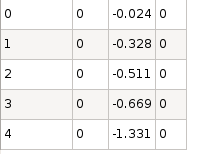
\includegraphics[width=0.3\textwidth]{\IMAGES/Part4_RANS/monitoring.png} 
\caption{Monitoring points coordinates}
\label{lag:cap1_monit}
\end{figure}
%
\figurename~\ref{lag:cap2_monit} presents the evolution of the velocity at the five monitoring points placed along the pipe axis at the z coordinates -0.024, -0.328, -0.511, -0.669 and -1.331m. This figure indicates that, after an intial transient during which the flow develops from the initial solution, the flow is well established and steady within 850 iterations. \figurename~\ref{lag:axial_velocity} shows a picture of the magnitude of the velocity at the outlet of the pipe.  
%
\begin{figure}[H]
\centering
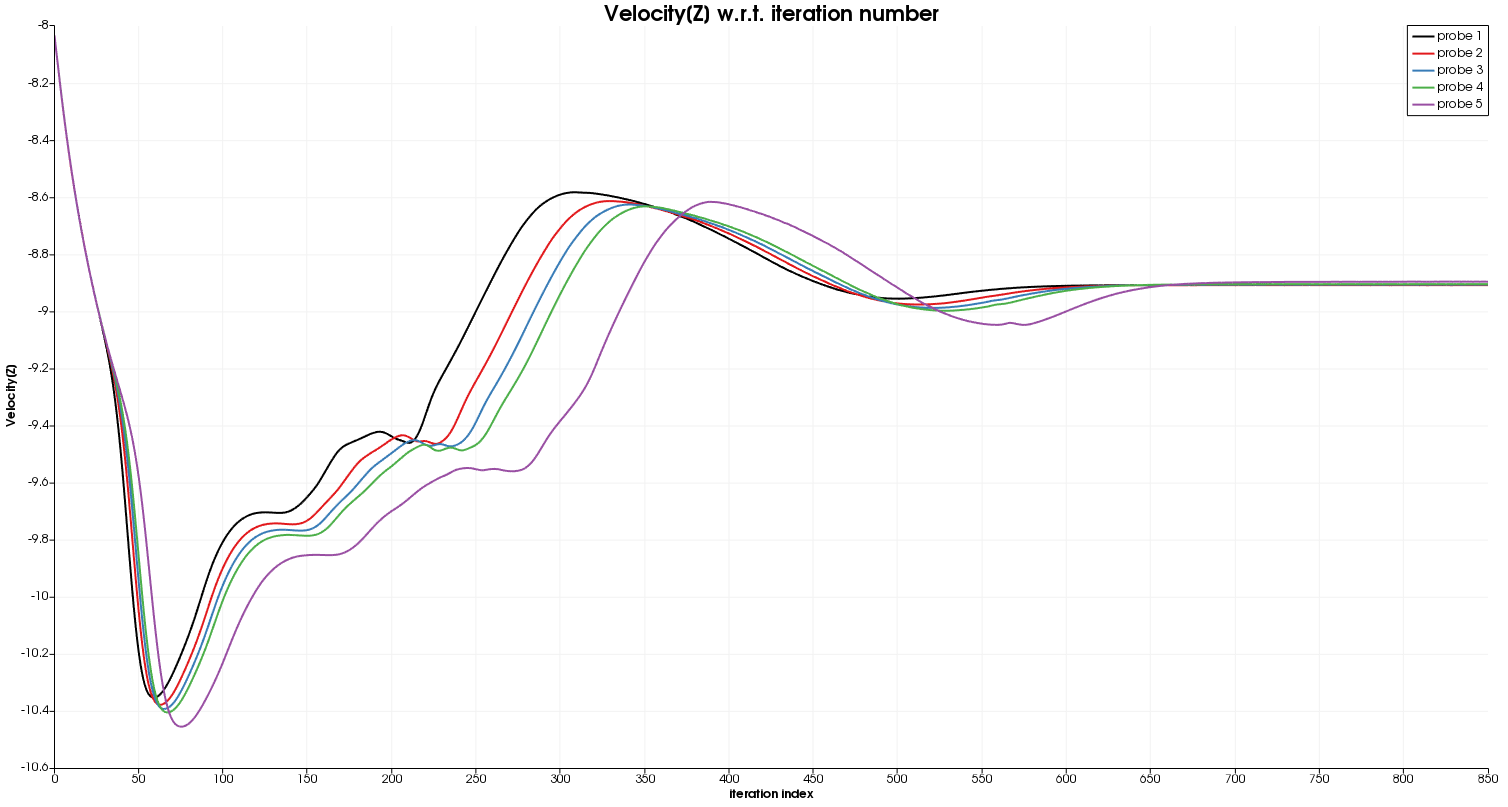
\includegraphics[width=0.8\textwidth]{\IMAGES/Part4_RANS/axial_velocity_conv.png}
\caption{Evolution of axial velocity during the calculation}
\label{lag:cap2_monit}
\end{figure}
%
\begin{figure}[H]
\centering
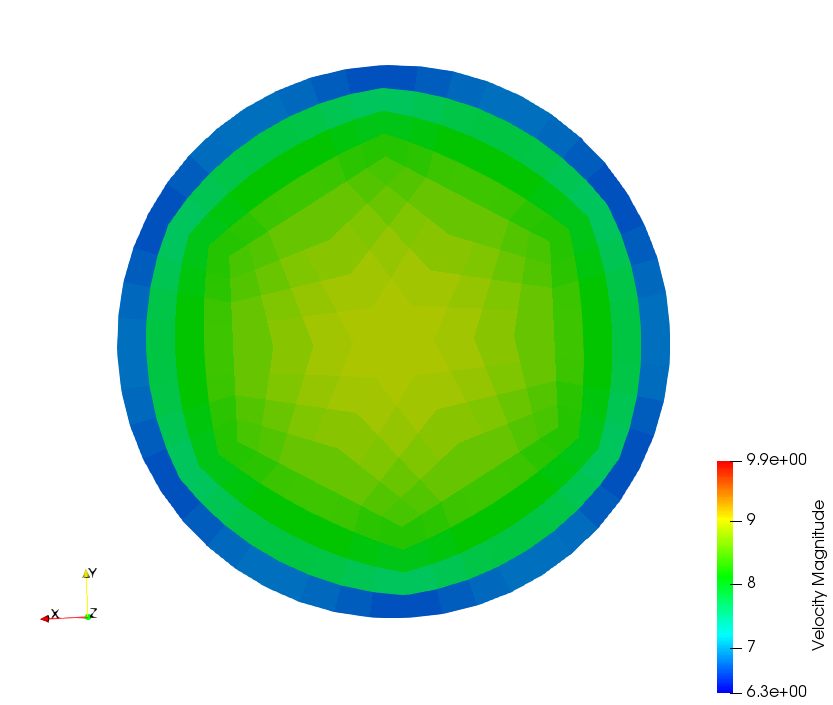
\includegraphics[width=0.5\textwidth]{\IMAGES/Part4_RANS/axial_velocity.png}
\caption{Velocity magnitude at outlet}
\label{lag:axial_velocity}
\end{figure}
%
Having generated the steady-state, single phase RANS flow field on which the particles will be injected, the first step of the one-way coupling, two phase Lagrangian \CS modelling of Arnason's \cite{Arnason} experiments has now been completed.  You can proceed to the setting-up, running, and analysis of the two phase Lagrangian \CS model.
